\section*{QUESTION 2}

\begin{center}
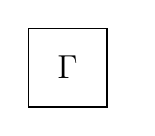
\begin{tikzpicture}
\node [draw,rectangle,minimum width=1cm,minimum height=1cm,label=right:$\Vdash $] (Gamma) {\large $\Gamma$};
\end{tikzpicture}
\end{center}
$\Gamma$ is the only possible world in this model that cannot access itself. It follows that $\Gamma \Vdash \bx P$ since $(\forall \Delta \in \mathcal{G})\ \Gamma\mathcal{R}\Delta \supset \Delta \Vdash P$ (When $\Delta \gets \Gamma$, the antecedent $\Gamma\mathcal{R}\Gamma$ is false so the conditional is true. Because there is only one world $\Gamma$, the universal quantification is true.). $\Gamma \not\Vdash \diam P$ since $(\exists \Delta \in \mathcal{G})\ \Gamma\mathcal{R}\Delta \land \Delta \Vdash P$ is false (When $\Delta \gets \Gamma$, the left conjunct $\Gamma\mathcal{R}\Gamma$ is false so the conjunction is false. Because there is only one world $\Gamma$, the existential quantification is false.). Consequently, $\Gamma \not\Vdash \bx P \supset \diam P$.